%!TEX root = ../../../main.tex

\subsection{IXMAS dataset}
    The IXMAS dataset was built by Perception project. It contains 12 action classes recorded by 4 side view cameras and 1 top view camera. 
    \begin{figure}[h]
        \centering
        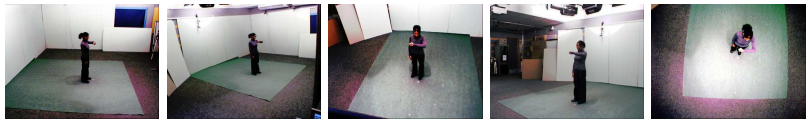
\includegraphics[width=1\linewidth]{figs/IXMAS1.png}
        \caption{Illustration of a frame extracted from an action observed by five camera viewpoints \cite{weinland2006free}}
        %\vspace{-0.3cm}
        \label{Fig:IXMAS1}
    \end{figure}
    Each action is performed 3 times by 10 actors (5 males / 5 females). %These actions are check watch, cross arms, scratch head, sit down, get up, turn around, walk, wave, punch, kick, point and pick up. 
    During the time of writing this paper, the dataset is not publicly provided due to the privacy issues. We have utilized a subset containing samples from four side camera views (excluding the top down view) that we have downloaded previously with agreement of the data-set's authors. The comparison with SOTA methods on this dataset will be only taken from the four side view cameras. 
